% <!-- coding: utf-8 -->
% http://www.cosmosportal.eu/cosmos/files/help/interactive_pdfs.pdf
\documentclass[a4paper,twoside,english]{article}
% \usepackage{minitoc}
\usepackage[utf8]{inputenc}
\usepackage[T1]{fontenc}
\usepackage[frenchb]{babel}
\usepackage{lmodern}% Choix de la fonte (Latin Modern de D. Knuth) %
\usepackage{textcomp} % pour l'euro
\usepackage{datetime}
% http://en.wikibooks.org/wiki/LaTeX/Page_Layout
% http://www.tex.ac.uk/tex-archive/info/apprends-latex/Apprends_LaTeX.pdf
\usepackage[top=2cm, bottom=2cm, left=0.5cm, right=0.5cm]{geometry}
% \DeclareGraphicsExtensions{.jpg,.mps,.pdf,.png} % Formats d'images
%
% mes personnalisations pour le document
\newcommand{\montitre}{Bretagne Vivante Rennes - Vilaine Aval}
\newcommand{\monlhead}{Bretagne Vivante Rennes - Vilaine Aval}
\newcommand{\malargeurgraphique}{93mm}
% les espaces en fin de ligne
\frenchspacing
% pour la planche contact
% http://en.wikibooks.org/wiki/LaTeX/Floats,_Figures_and_Captions
% \usepackage[demo]{graphicx}
\usepackage{graphicx}
\usepackage{caption}
%
\usepackage{subcaption}
% http://www.peteryu.ca/tutorials/publishing/latex_captions
\captionsetup[subfigure]{labelformat=empty}
% pour supprimer la numérotation
% \renewcommand{\thesubfigure}{\arabic{subfigure}}
\renewcommand{\thesubfigure}{}
%
% la séparation entre les figures
% http://newsgroups.derkeiler.com/Archive/Comp/comp.text.tex/2010-08/msg00435.html
\setlength{\textfloatsep}{0pt}
\setlength{\floatsep}{0pt}
% la date en francais
\usepackage{datetime}
\newdateformat{mydate}{\THEDAY/\THEMONTH/\THEYEAR}
%
% la personnalisation des entête/pied de page
\usepackage{fancyhdr}
\usepackage{lastpage}
\fancyhf{}
\fancyhead[LO,RE]{\fontsize{14}{16}\selectfont\monlhead}
\fancyhead[LE,RO]{\fontsize{14}{16}\selectfont\montitre}
\pagestyle{fancy}
\renewcommand\sectionmark[1]{\markboth{\MakeUppercase{#1}}{}}
\rfoot{\thepage/\pageref{LastPage}}
\cfoot{Matthieu Beaufils \& Marc Gauthier}
\lfoot{\mydate\today}
% on supprime la ligne en dessous de l'entête
\renewcommand{\headrulewidth}{0pt}

%
% pour les deux colonnes
\usepackage{supertabular}
%
% pour les trois colonnes
\usepackage{multicol}
% pour améliorer les tableaux
\usepackage{array}
%

% http://tex.stackexchange.com/questions/66252/placing-the-figure-exactly-at-the-top-of-the-page-in-latex
\makeatletter
\setlength{\@fptop}{0pt}
\makeatother
% http://tex.stackexchange.com/questions/42968/reduction-of-space-between-two-sub-figures
% \usepackage{showframe}
%
% pour les tables des matières
% http://tex.stackexchange.com/questions/186515/remove-chapter-number-from-minitoc
% \newcommand{\filterminitoc}[1]{#1}
% \renewcommand{\thesection}{\csname filterminitoc \endcsname{\arabic{chapter}.}\arabic{section}}
% \newcommand{\minitocsection}{\begingroup\renewcommand{\filterminitoc}[1]{}\minitoc\endgroup}
\newcommand{\HRule}{\rule{\linewidth}{0.5mm}}
% pour les carrés de couleur
\usepackage{xcolor}

\usepackage{titlesec}
\titlespacing*{\subsubsection}{0pt}{5pt}{0pt}
\usepackage{hyperref}
\hypersetup{
   pdfauthor   = {Marc Gauthier},
   colorlinks=true,
   breaklinks=true,
   urlcolor= blue,
   linkcolor= blue,
   linkbordercolor=blue,
   pdfcreator  = {\LaTeX},
}
\newcommand\crule[3][black]{\textcolor{#1}{\rule{#2}{#3}}}
% les espaces en fin de ligne
\frenchspacing
% http://daniel.flipo.free.fr/frenchb/frenchb-doc.pdf
% http://borntocode.fr/latex-customisation-de-listes-a-puces/
% https://en.wikibooks.org/wiki/LaTeX/List_Structures
% \frenchbsetup{StandardItemizeEnv=true, StandardEnumerateEnv=true, ReduceListSpacing=true, ItemLabels=\textendash}
% pour avoir les versions des modules
\listfiles
\begin{document}
%
% la page de garde
% http://www.jujens.eu/posts/2013/Oct/20/latex-page-garde/
\begin{titlepage}
  \begin{sffamily}
  \begin{center}

    % Upper part of the page. The '~' is needed because \\
    % only works if a paragraph has started.


    \textsc{\LARGE Bretagne Vivante Rennes}\\[1cm]
    \textsc{\Large Vilaine Aval - oiseaux en hiver}\\[1cm]

    % Title
    \HRule \\[0.4cm]
    { \huge \bfseries Données serena}
    \HRule \\[0.4cm]
    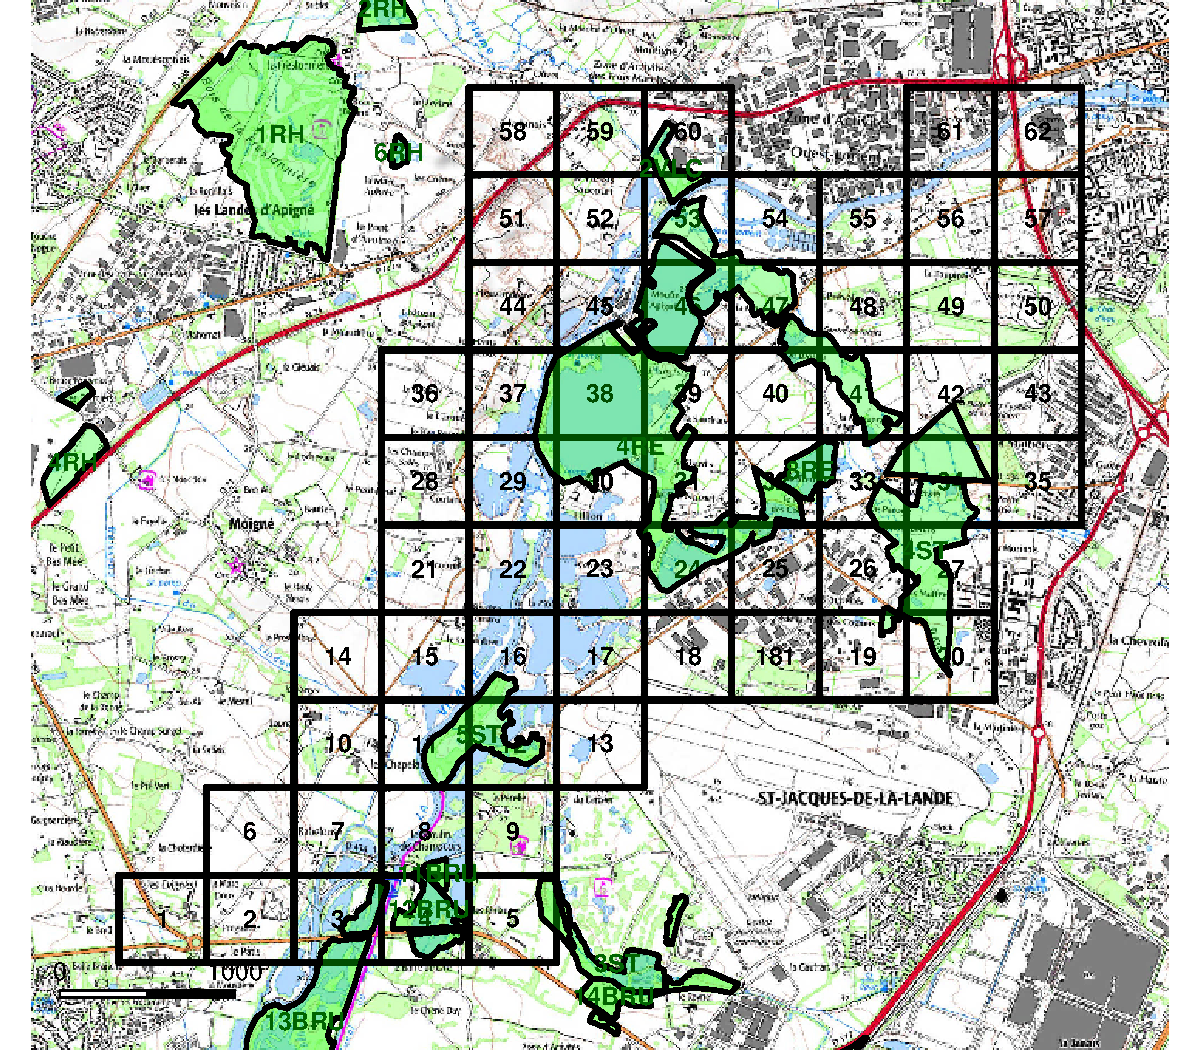
\includegraphics[width=190mm]{territoire_Nord.pdf}~\\[.5cm]
    \HRule \\[0.4cm]
    \begin{minipage}{0.4\textwidth}
      \begin{flushleft} \large
        \emph{Coordination}\\
        Matthieu Beaufils\\
         Marc Gauthier
      \end{flushleft}
    \end{minipage}
    \begin{minipage}{0.4\textwidth}
      \begin{flushright} \large
        \emph{Informatique}\\
        Marc Gauthier
      \end{flushright}
    \end{minipage}

    \vfill
  \end{center}
  \end{sffamily}
\end{titlepage}
\setlength{\parskip}{0pt} % 1ex plus 0.5ex minus 0.2ex}
\setlength{\parindent}{0pt}
\twocolumn
% <!-- coding: utf-8 -->
\renewcommand{\monlhead}{Parcours}
\section{Parcours}
Un parcours dure 5 minutes, ce qui correspond à 333 mètres à 4 km/h.

Suivant le terrain et la densité d'oiseaux, cette longueur peut variée.

En cas de difficulté d'identification d'oiseaux (roitelet par exemple), la durée est augmentée.

Pour les points d'écoute, la longueur est nulle.

Les parcours sont enregistrés en format geojson. Les données sont ensuite traitées en R

\subsection{par observateur}
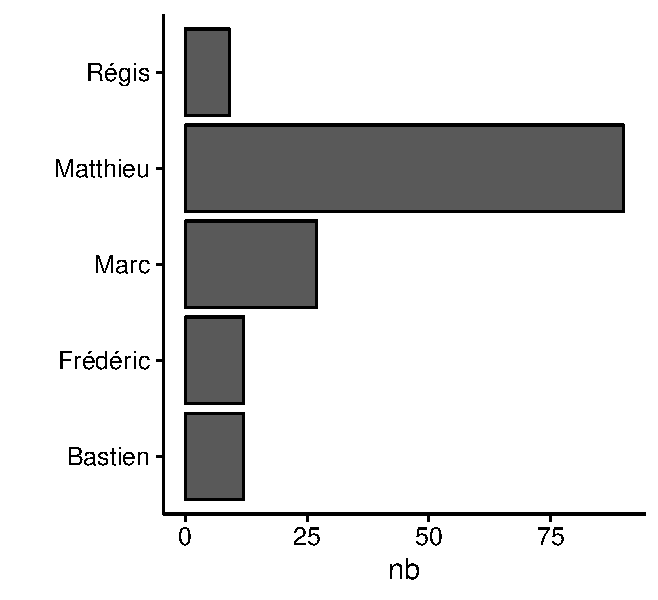
\includegraphics[width=\malargeurgraphique]{images/parcours_stat_champ_prenom.pdf}
\subsection{par longueur}
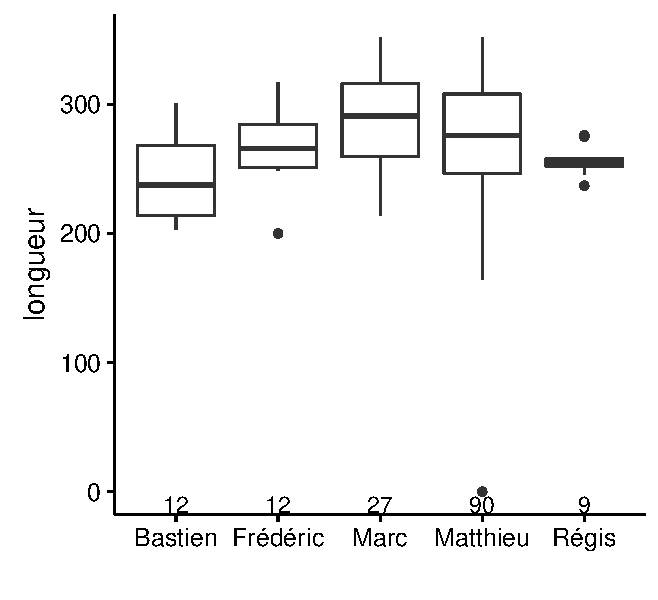
\includegraphics[width=\malargeurgraphique]{images/parcours_stat_email_longueur.pdf}
\subsection{carte}
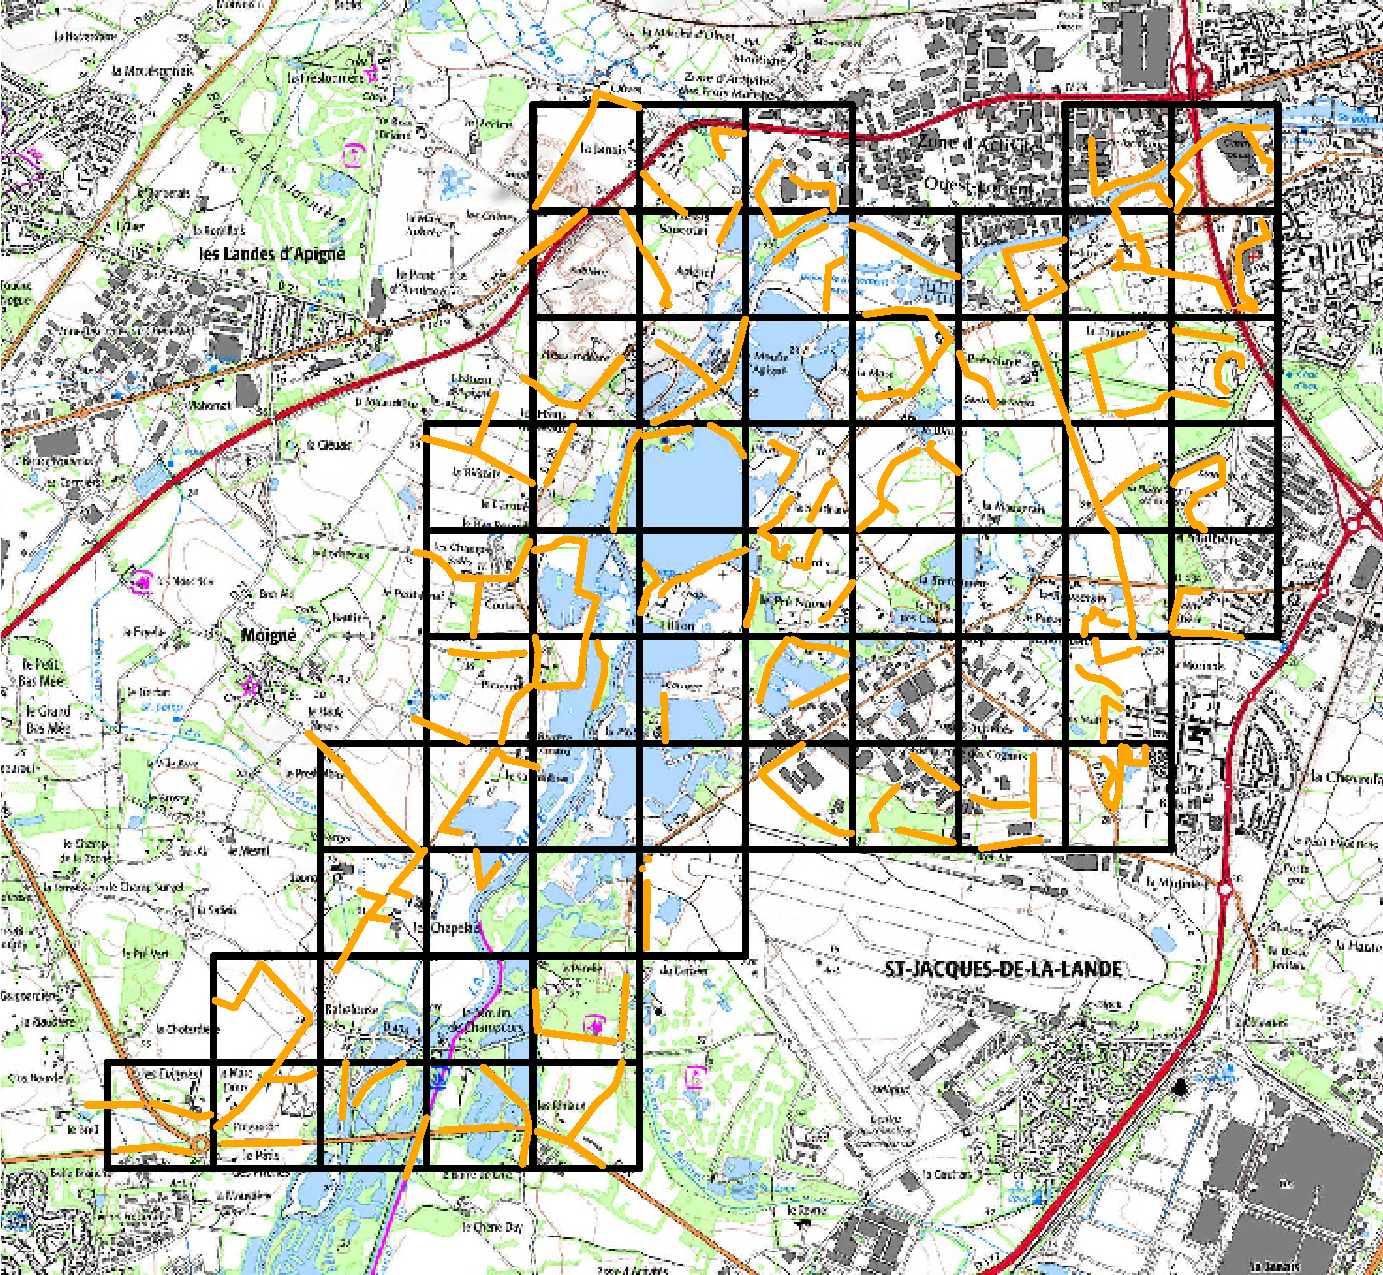
\includegraphics[width=\malargeurgraphique]{images/parcours_carte.pdf}
\clearpage

% <!-- coding: utf-8 -->
\renewcommand{\monlhead}{Données serena}
\section{Données serena}
Les données sont extraites de serena

Cette extraction est faite en format xls. Les données sont ensuite traitées en R :
\begin{itemize}
\item suppression des données "Hors protocole"
\item normalisation du champ OBSE PLACE
\item détermination de la maille à partir du champ OBSE PLACE
\item détermination de la maille à partir des coordonnées géographiques
\end{itemize}

\subsection{par espèce}
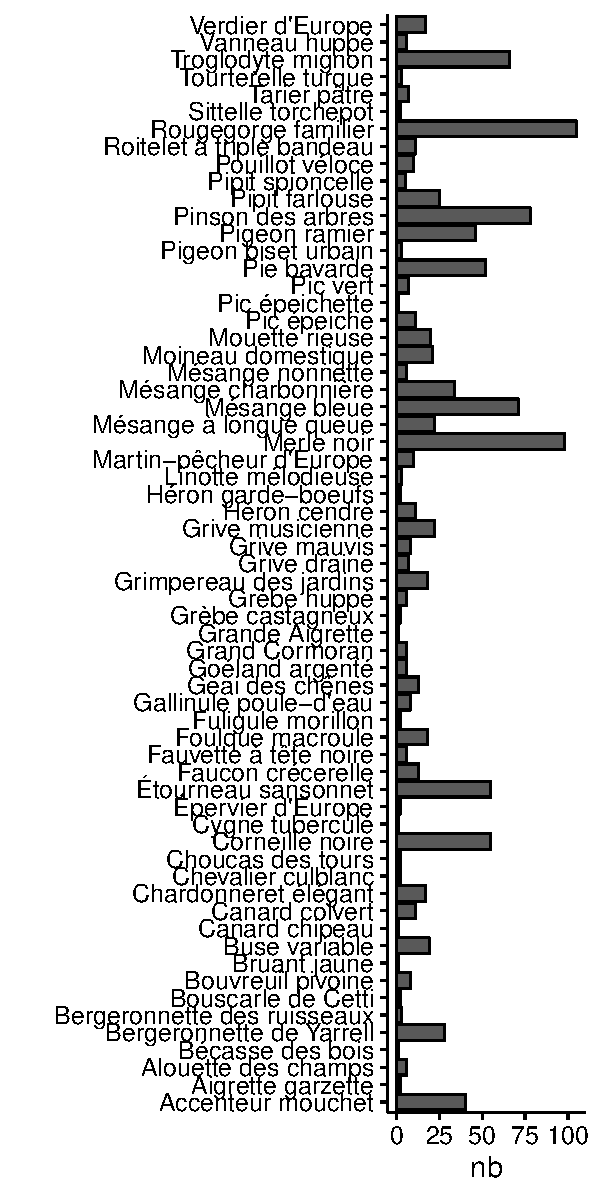
\includegraphics[width=\malargeurgraphique]{images/serena_stat_champ_espece.pdf}
\subsection{par date}
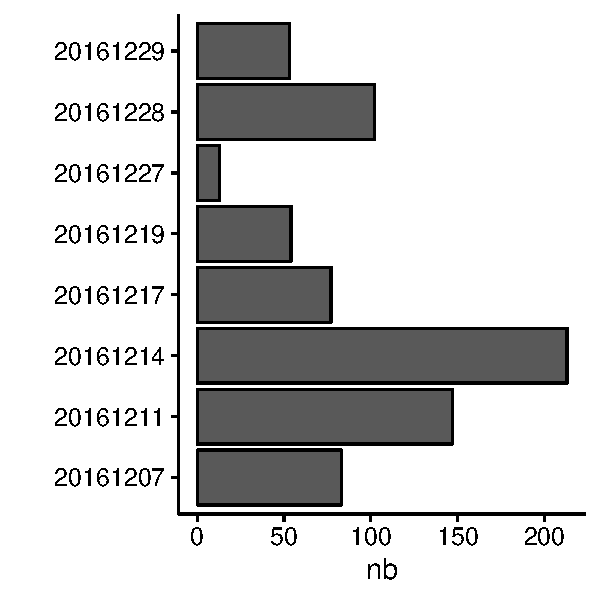
\includegraphics[width=\malargeurgraphique]{images/serena_stat_champ_OBSE_DATE.pdf}
\subsection{par observateur}
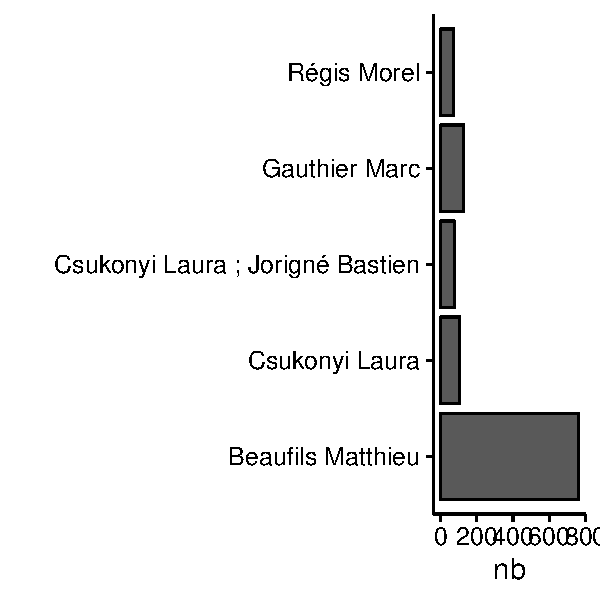
\includegraphics[width=\malargeurgraphique]{images/serena_stat_champ_OBSV_LIBEL.pdf}
\onecolumn
\subsection{carte parcours}
Le parcours est localisé en fonction de ses coordonnées.

En noir, les parcours avec une incohérence maille.
\begin{figure}[!h]
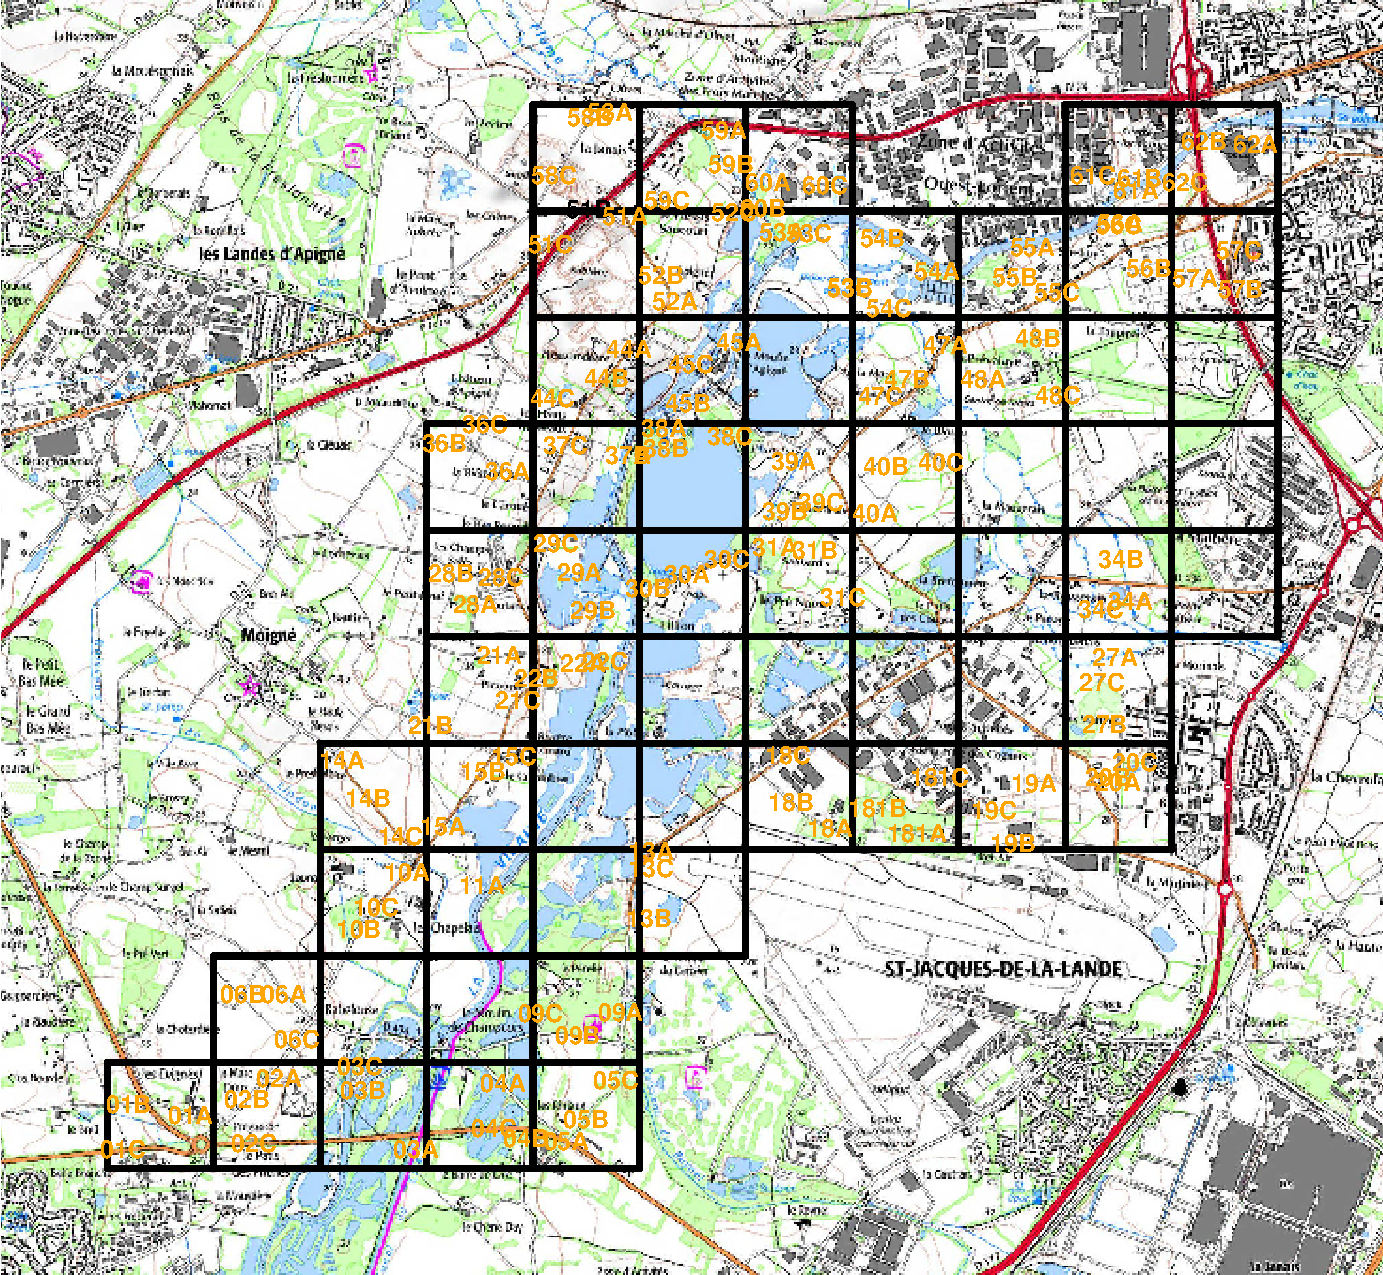
\includegraphics[width=1.0\textwidth]{images/serena_carte.pdf}
\end{figure}
\clearpage
\subsection{carte statistiques}
Pour chaque maille, on a le nombre de :
\begin{itemize}
\item parcours"
\item espèces
\item données
\end{itemize}
\begin{figure}[!h]
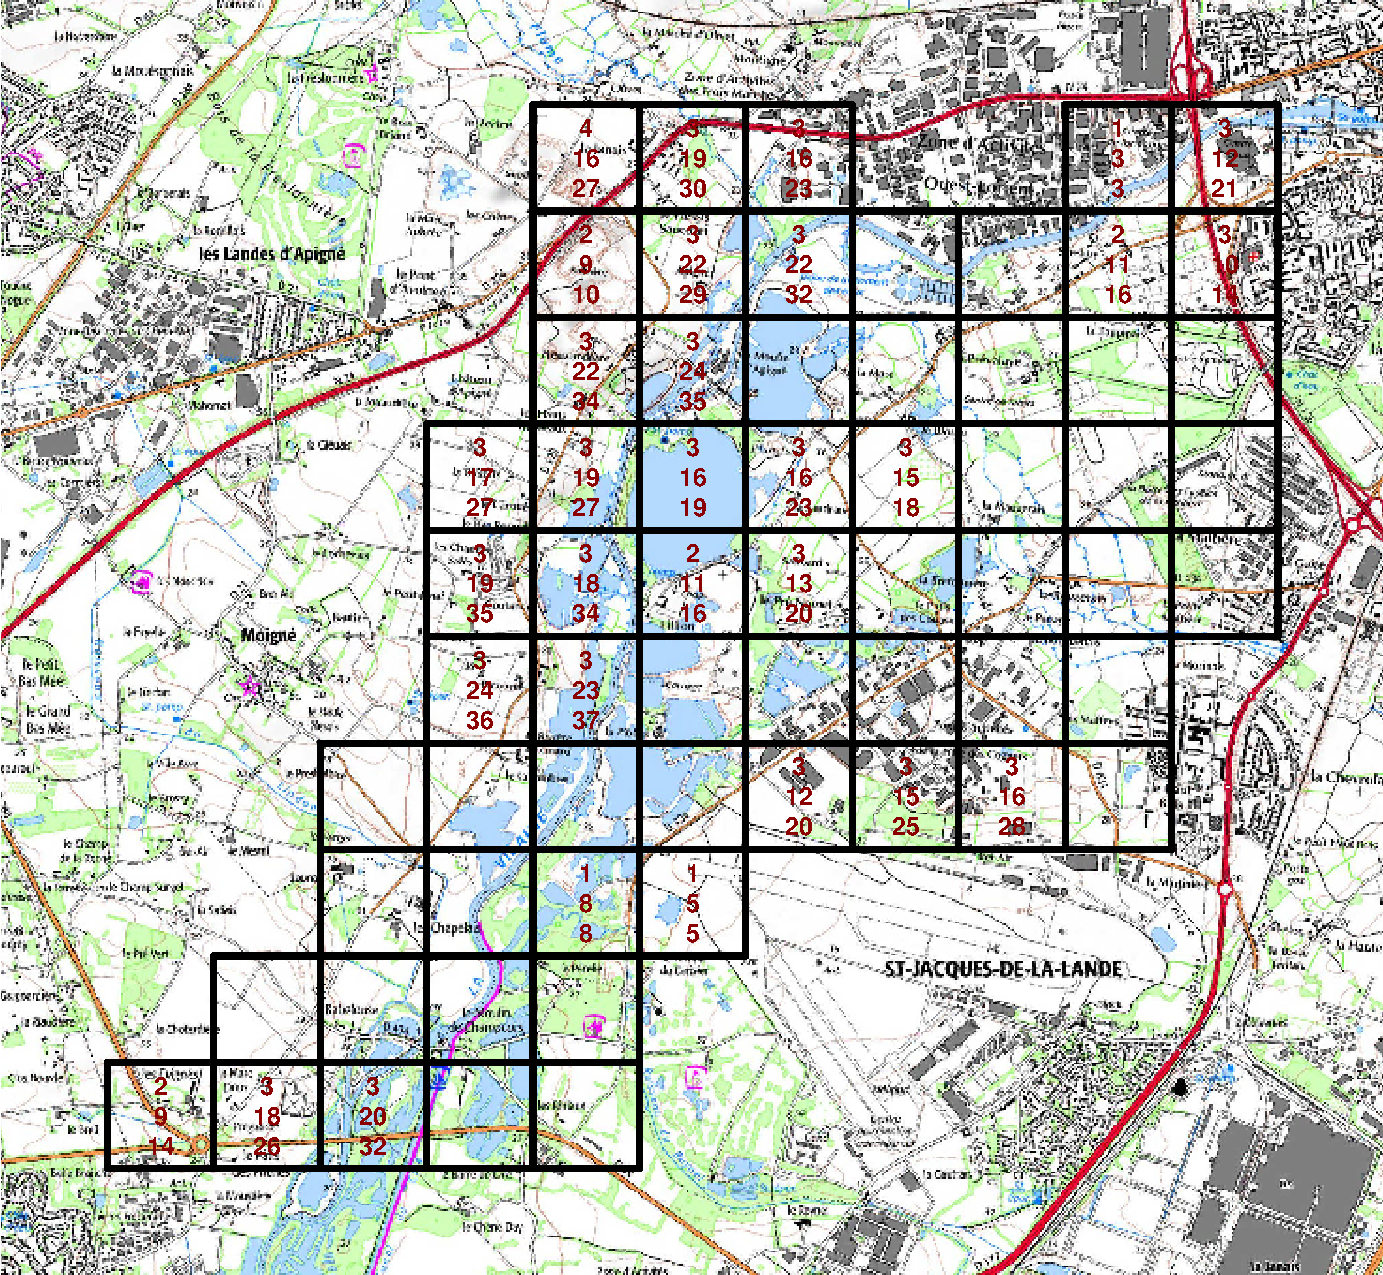
\includegraphics[width=1.0\textwidth]{images/serena_carte_stat.pdf}
\end{figure}
\clearpage
\twocolumn
\section{Atlas par espèce}
\clearpage
% <!-- coding: utf-8 -->
\subsection{Accenteur mouchet}
\includegraphics[width=\malargeurgraphique]{atlas_serena/AccenteurMouchet.pdf}
\subsection{Alouette des champs}
\includegraphics[width=\malargeurgraphique]{atlas_serena/AlouetteDesChamps.pdf}
\subsection{Bécasse des bois}
\includegraphics[width=\malargeurgraphique]{atlas_serena/BecasseDesBois.pdf}
\subsection{Bergeronnette des ruisseaux}
\includegraphics[width=\malargeurgraphique]{atlas_serena/BergeronnetteDesRuisseaux.pdf}
\subsection{Bergeronnette de Yarrell}
\includegraphics[width=\malargeurgraphique]{atlas_serena/BergeronnetteDeYarrell.pdf}
\subsection{Bouscarle de Cetti}
\includegraphics[width=\malargeurgraphique]{atlas_serena/BouscarleDeCetti.pdf}
\subsection{Bouvreuil pivoine}
\includegraphics[width=\malargeurgraphique]{atlas_serena/BouvreuilPivoine.pdf}
\subsection{Buse variable}
\includegraphics[width=\malargeurgraphique]{atlas_serena/BuseVariable.pdf}
\subsection{Canard chipeau}
\includegraphics[width=\malargeurgraphique]{atlas_serena/CanardChipeau.pdf}
\subsection{Canard colvert}
\includegraphics[width=\malargeurgraphique]{atlas_serena/CanardColvert.pdf}
\subsection{Chardonneret élégant}
\includegraphics[width=\malargeurgraphique]{atlas_serena/ChardonneretElegant.pdf}
\subsection{Chevalier culblanc}
\includegraphics[width=\malargeurgraphique]{atlas_serena/ChevalierCulblanc.pdf}
\subsection{Choucas des tours}
\includegraphics[width=\malargeurgraphique]{atlas_serena/ChoucasDesTours.pdf}
\subsection{Corneille noire}
\includegraphics[width=\malargeurgraphique]{atlas_serena/CorneilleNoire.pdf}
\subsection{Étourneau sansonnet}
\includegraphics[width=\malargeurgraphique]{atlas_serena/EtourneauSansonnet.pdf}
\subsection{Faucon crécerelle}
\includegraphics[width=\malargeurgraphique]{atlas_serena/FauconCrecerelle.pdf}
\subsection{Fauvette à tête noire}
\includegraphics[width=\malargeurgraphique]{atlas_serena/FauvetteATeteNoire.pdf}
\subsection{Foulque macroule}
\includegraphics[width=\malargeurgraphique]{atlas_serena/FoulqueMacroule.pdf}
\subsection{Fuligule morillon}
\includegraphics[width=\malargeurgraphique]{atlas_serena/FuliguleMorillon.pdf}
\subsection{Gallinule poule-d’eau}
\includegraphics[width=\malargeurgraphique]{atlas_serena/GallinulePouleDEau.pdf}
\subsection{Geai des chênes}
\includegraphics[width=\malargeurgraphique]{atlas_serena/GeaiDesChenes.pdf}
\subsection{Goéland argenté}
\includegraphics[width=\malargeurgraphique]{atlas_serena/GoelandArgente.pdf}
\subsection{Grand Cormoran}
\includegraphics[width=\malargeurgraphique]{atlas_serena/GrandCormoran.pdf}
\subsection{Grèbe castagneux}
\includegraphics[width=\malargeurgraphique]{atlas_serena/GrebeCastagneux.pdf}
\subsection{Grèbe huppé}
\includegraphics[width=\malargeurgraphique]{atlas_serena/GrebeHuppe.pdf}
\subsection{Grimpereau des jardins}
\includegraphics[width=\malargeurgraphique]{atlas_serena/GrimpereauDesJardins.pdf}
\subsection{Grive draine}
\includegraphics[width=\malargeurgraphique]{atlas_serena/GriveDraine.pdf}
\subsection{Grive mauvis}
\includegraphics[width=\malargeurgraphique]{atlas_serena/GriveMauvis.pdf}
\subsection{Grive musicienne}
\includegraphics[width=\malargeurgraphique]{atlas_serena/GriveMusicienne.pdf}
\subsection{Héron cendré}
\includegraphics[width=\malargeurgraphique]{atlas_serena/HeronCendre.pdf}
\subsection{Linotte mélodieuse}
\includegraphics[width=\malargeurgraphique]{atlas_serena/LinotteMelodieuse.pdf}
\subsection{Martin-pêcheur d'Europe}
\includegraphics[width=\malargeurgraphique]{atlas_serena/MartinPecheurDEurope.pdf}
\subsection{Merle noir}
\includegraphics[width=\malargeurgraphique]{atlas_serena/MerleNoir.pdf}
\subsection{Mésange à longue queue}
\includegraphics[width=\malargeurgraphique]{atlas_serena/MesangeALongueQueue.pdf}
\subsection{Mésange bleue}
\includegraphics[width=\malargeurgraphique]{atlas_serena/MesangeBleue.pdf}
\subsection{Mésange charbonnière}
\includegraphics[width=\malargeurgraphique]{atlas_serena/MesangeCharbonniere.pdf}
\subsection{Mésange nonnette}
\includegraphics[width=\malargeurgraphique]{atlas_serena/MesangeNonnette.pdf}
\subsection{Moineau domestique}
\includegraphics[width=\malargeurgraphique]{atlas_serena/MoineauDomestique.pdf}
\subsection{Mouette rieuse}
\includegraphics[width=\malargeurgraphique]{atlas_serena/MouetteRieuse.pdf}
\subsection{Pic épeiche}
\includegraphics[width=\malargeurgraphique]{atlas_serena/PicEpeiche.pdf}
\subsection{Pic épeichette}
\includegraphics[width=\malargeurgraphique]{atlas_serena/PicEpeichette.pdf}
\subsection{Pic vert}
\includegraphics[width=\malargeurgraphique]{atlas_serena/PicVert.pdf}
\subsection{Pie bavarde}
\includegraphics[width=\malargeurgraphique]{atlas_serena/PieBavarde.pdf}
\subsection{Pigeon biset urbain}
\includegraphics[width=\malargeurgraphique]{atlas_serena/PigeonBisetUrbain.pdf}
\subsection{Pigeon ramier}
\includegraphics[width=\malargeurgraphique]{atlas_serena/PigeonRamier.pdf}
\subsection{Pinson des arbres}
\includegraphics[width=\malargeurgraphique]{atlas_serena/PinsonDesArbres.pdf}
\subsection{Pipit farlouse}
\includegraphics[width=\malargeurgraphique]{atlas_serena/PipitFarlouse.pdf}
\subsection{Pipit spioncelle}
\includegraphics[width=\malargeurgraphique]{atlas_serena/PipitSpioncelle.pdf}
\subsection{Pouillot véloce}
\includegraphics[width=\malargeurgraphique]{atlas_serena/PouillotVeloce.pdf}
\subsection{Roitelet à triple bandeau}
\includegraphics[width=\malargeurgraphique]{atlas_serena/RoiteletATripleBandeau.pdf}
\subsection{Rougegorge familier}
\includegraphics[width=\malargeurgraphique]{atlas_serena/RougegorgeFamilier.pdf}
\subsection{Sittelle torchepot}
\includegraphics[width=\malargeurgraphique]{atlas_serena/SittelleTorchepot.pdf}
\subsection{Tarier pâtre}
\includegraphics[width=\malargeurgraphique]{atlas_serena/TarierPatre.pdf}
\subsection{Tarier pâtre}
\includegraphics[width=\malargeurgraphique]{atlas_serena/TarierPatre.pdf}
\subsection{Tourterelle turque}
\includegraphics[width=\malargeurgraphique]{atlas_serena/TourterelleTurque.pdf}
\subsection{Troglodyte mignon}
\includegraphics[width=\malargeurgraphique]{atlas_serena/TroglodyteMignon.pdf}
\subsection{Vanneau huppé}
\includegraphics[width=\malargeurgraphique]{atlas_serena/VanneauHuppe.pdf}
\subsection{Verdier d'Europe}
\includegraphics[width=\malargeurgraphique]{atlas_serena/VerdierDEurope.pdf}


\onecolumn
\end{document}